\documentclass[10pt,a4paper]{article}
\usepackage[margin=2.2cm]{geometry}
\usepackage{graphicx}
\usepackage{booktabs}
\usepackage{amsmath}
\usepackage{caption}
\usepackage{subcaption}
\usepackage{xcolor}
\usepackage[hidelinks]{hyperref}
\usepackage{enumitem}
\usepackage{float}
\setlist{nosep,leftmargin=1.4em}
\captionsetup{font=small,labelfont=bf}
\newcommand{\todo}[1]{\textcolor{red}{[#1]}}
\newcommand{\doi}[1]{\href{https://doi.org/#1}{\nolinkurl{doi:#1}}}

\title{Replicating and extending the analysis of Braboszcz et al.\ (2017) on OpenNeuro \texttt{ds003969}}
\date{October 2026}

\begin{document}
\maketitle

\begin{abstract}
We replicate the EEG analysis of Braboszcz et al.\ (2017), who reported higher gamma (60--110\,Hz) power in meditators
from three traditions than in controls, higher alpha power in Vipassana practitioners, and a correlation between
gamma power and meditation experience. Using the public OpenNeuro dataset \texttt{ds003969}, we rebuilt their pipeline
in MNE-Python, replacing manual preprocessing steps with automated equivalents. Without ICA,
our per-subject parieto-occipital gamma closely matches the paper's own values ($r = 0.97$). The gamma and alpha
group differences replicate, with or without automated ICA, though ICA weakens the gamma effect for Vipassana
practitioners. The correlation between gamma and log practice hours reproduces exactly ($r = 0.33$),
but only after removing two outliers. When outlier detection is repeated within the bootstrap, the confidence
interval includes zero, and our own gamma values show no relationship. We then extend the analysis to criticality,
measuring long-range temporal correlations (DFA) and functional excitation/inhibition balance (fEI). DFA shows no
differences between meditators and controls, consistent with recent work. Vipassana practitioners show higher alpha
fEI, which closely tracks their higher alpha power. Beta DFA rises from the first to the second meditation block, but
this cannot be separated from a generic time-on-task effect. These results are robust to removing ICA and to using
shorter analysis epochs.
\end{abstract}

%-------------------------------------------------------------------------------
\section{Introduction}

In an effort to learn more about EEG preprocessing and analysis, this project aimed to replicate and 
extend the findings of Braboszcz et al.\ (2017) using the OpenNeuro dataset \texttt{ds003969}. This paper 
analyses EEG recordings for meditators from 3 different traditions alongside controls, across meditation and
instructed mind-wandering conditions. Analysis focused on spectral power differences and their relationship 
to meditation experience.

To be clear, this is a replication of the analysis and EEG preprocessing of Braboszcz et al.\ (2017), 
using the publicly available dataset \texttt{ds003969} which they released, rather than a replication of 
their result on different data.

In addition to replicating the original findings, this project incorporated additional analysis looking at 
criticality measures,
inspired by Lewis-Healey et al. (2026)'s recent findings on effort(lessness) and criticality during meditation. 
Criticality measures used were based on the detrended fluctuation analysis (DFA) framework of Linkenkaer-Hansen et al.\ (2001) and Hardstone et al.\ (2012)
with functional excitation/inhibition balance (fEI) providing another complementary measure, based on the
approach of Bruining et al.\ (2020).

The concrete tasks were:
\begin{itemize}
  \item \textbf{Build an equivalent pipeline in MNE-Python}, matching the authors' description of their MATLAB pipeline
       as closely as the text allows.
  \item \textbf{Replicate the headline results on spectral power:}
        \begin{itemize}
          \item higher parieto-occipital gamma (60--110\,Hz) in each meditator group than in controls, as a trait
                and during MED;
          \item higher alpha (7--11\,Hz) for Vipassana practitioners than in each of the other groups during meditation;
          \item higher parieto-occipital gamma for meditators correlated with log lifetime practice hours.
        \end{itemize}
  \item \textbf{Extend the analysis to criticality.} Compute long-range temporal correlations (DFA) and functional
        excitation/inhibition balance (fEI), testing the hypotheses that:
      \begin{itemize}
          \item DFA and fEI have no trait differences between meditators and controls;
          \item DFA increases over time during meditation.
        \end{itemize}
\end{itemize}

\section{The original paper}

\label{sec:paper}

Braboszcz et al. (2017) recorded EEG data from experienced meditators and non-meditator controls, across 
meditation and instructed mind-wandering conditions. Experienced meditators came from three different
meditation traditions: Himalayan Yoga, Isha Shoonya, and Vipassana. 

Their analysis focuses on differences in resting state EEG spectral power in particular frequency bands between
meditators and controls. Finding some significant differences, they go on to find a relationship between
the difference in gamma power observed in meditators and lifetime hours of meditative practice.

\paragraph{Participants and setting.} Data were collected at the Meditation Research Institute in Rishikesh,
India. Meditators were recruited for their expertise in one of three traditions:
\begin{itemize}
  \item \textbf{Himalayan Yoga (HYT):} silent mantra repetition, with or without breath awareness.
  \item \textbf{Isha Shoonya (ISY):} a practice of conscious ``non-doing'' with no object of focus.
  \item \textbf{Vipassana (VIP, S.\,N.\ Goenka style):} scanning the body from head to toes and back, observing
        sensations with equanimity.
      \item \textbf{Transcendental Meditation (TM):} a practice involving the silent repetition of a mantra, 
      typically for 20 minutes twice a day. These were excluded from the main analysis as there were only a few participants practicing TM.
\end{itemize}
Controls (CTR) had no meditation practice. From a reported 99 people recruited (27 HYT, 20 ISY, 20 VIP, 32 CTR), 
the authors formed four groups of 16, matched on age and gender, for 64 in total. 
Mean ages were 40--49 per group and did not differ significantly. HYT and VIP had more lifetime practice 
than ISY (means of roughly 15{,}000 and 9{,}000 hours against 2{,}600).

\paragraph{Design.} Each participant did two 20-minute blocks, with eyes closed in a dark, soundproof room:
\begin{itemize}
  \item \textbf{Meditation (MED):} 10 minutes of breath focus, then 10 minutes of the participant's own practice,
        cued over an intercom. Controls continued breath focus for the second half.
  \item \textbf{Instructed mind-wandering (IMW):} recalling autobiographical events from childhood to the recent
        past, avoiding emotionally charged memories.
\end{itemize}
Block order was counterbalanced within each group, and participants filled in questionnaires between the two blocks.
Auditory and visual tasks were also run in the sessions; their results are not reported in the paper.
EEG was recorded with a 64-channel Biosemi ActiveTwo system at 1024\,Hz, with mastoid and EOG electrodes.
The analysis compared the last 10 minutes of MED with the last 10 minutes of IMW.

\paragraph{Analysis.} Recordings were referenced to the right mastoid, downsampled to 256\,Hz and high-pass filtered
at 1\,Hz. Artefactual segments were rejected with EEGLAB's \texttt{pop\_rejcont}, bad channels were removed by
eye, and 1--5 eye and temporal-muscle ICA components per subject were removed after visual inspection. Spectra were
computed from 1\,s epochs and compared with cluster permutation tests over electrodes and Welch or mixed ANOVAs.

\paragraph{Findings.}
\begin{itemize}
  \item \textbf{Gamma (60--110\,Hz):} all three meditator groups had higher parieto-occipital power than controls,
        both as a trait (MED and IMW combined) and during MED.
  \item \textbf{Alpha (7--11\,Hz):} VIP had more power than each of the other three groups, during MED and IMW.
  \item \textbf{Experience:} parieto-occipital gamma correlated with log lifetime practice hours ($r=0.33$; their Fig.~4D).
  \item \textbf{Artefact controls:} temporal-muscle components did not correlate with gamma. Eye-movement
        components did ($r=0.33$), but they did not correlate with experience, and the authors concluded that
        artefacts were unlikely to explain the gamma findings.
\end{itemize}
The paper's spectra by group are reproduced in Fig.~\ref{fig:paper}.

%-------------------------------------------------------------------------------

\section{Data}
\label{sec:data}

\paragraph{The dataset.} OpenNeuro \texttt{ds003969} (v1.0.0) contains 64-channel Biosemi recordings of 98
participants: 31 CTR, 24 HYT (``HTR'' in the dataset), 20 ISY (``SNY''), 19 VIP and 4 Transcendental Meditation. 
These counts don't line up exactly with those reported in the paper.
Each participant's two sessions are recorded in four $\sim$10-minute BDF files: \texttt{think1}, \texttt{think2},
\texttt{med1breath} (breath focus) and \texttt{med2} (the tradition's own practice; breath focus for controls).
The paper's analysis periods are therefore \texttt{think2} (IMW) and \texttt{med2} (MED).
Due to a defect, electrode \texttt{Fp1} is replaced by \texttt{EXG8}, the spare electrode wired in its place.

\paragraph{Session timing.} The recording start times in the BDF headers show how the blocks were scheduled. Both
blocks of a session were recorded back to back, and the two sessions were separated by a
median of 66\,minutes (range 47--89), all on one day. Roughly half of the participants did the MED session first (51 of 98) and half
the IMW session first (47), as recorded in the \texttt{first\_session} column of \texttt{participants.tsv}; this agrees
with the timestamps for all 98. Within a session the order is fixed, so \texttt{med2} always directly follows
\texttt{med1breath}. 

\paragraph{The paper's subject list (Zenodo).} The dataset does not record which 64 participants the paper analysed.
The authors' earlier Zenodo deposit (doi 10.5281/zenodo.57911) lists them by lab ID, with their per-subject median
parieto-occipital gamma and alpha values. We mapped these lab IDs to \texttt{ds003969} subjects using the recording
dates in the BDF headers, cross-checked against age. 63 of the 64 are in \texttt{ds003969}; HYT26's recording is 
missing from the publicly released data. All results in this report use this matched sample (16 CTR, 15 HYT, 16 ISY, 16 VIP, 252
recordings). The paper's per-subject
values are also used directly, to check the replication subject by subject. 

%-------------------------------------------------------------------------------

\section{Methodology}

\subsection{Pipeline replication}
\label{sec:process}

Table~\ref{tab:pipeline} sets the paper's description against what was implemented. Every step was
either matched as closely as the text allows.
In cases where manual decisions were made for e.g. artefact or bad channel detection, 
these were replaced by an automated equivalent. Initially we attempted to reconstruct
these manual judgements on bad channels and bad ICA components, but it quickly 
became clear that we were not able to make the same manual judgements reliably.

Counts in the table are for the 252 matched-sample recordings.

\begin{table}[h]
\centering\small
\begin{tabular}{@{}p{2.6cm}p{6.2cm}p{6.6cm}@{}}
\toprule
Step & Paper & This replication \\
\midrule
Sample & 16 per group, matched on age and gender from a larger pool; TM not included &
  The paper's matched list, 63 of 64 available (See section~\ref{sec:data}) \\
Reference & Right mastoid & Right mastoid (\texttt{EXG6}) \\
Resample, filter & 256\,Hz; 1\,Hz IIR high-pass, order 6, 0.3\,Hz transition & Same \\
Segment rejection & EEGLAB \texttt{pop\_rejcont}: 1\,s epochs, 0.5\,s overlap, 0--10\,Hz $>$17\,dB, 35--128\,Hz $>$14\,dB, contiguous 8;
  thresholds ``in rare cases'' adjusted by 1--5\,dB after visual review &
  Line-by-line Python port with unit tests, including EEGLAB quirks such as \texttt{contiguous} acting as a merge distance.
  Underspecified manual threshold adjustment not reproduced. \\
Bad channels & Manual; 0--18 per subject, mean $\approx$5; interpolation not stated &
  Automated: union of MNE waveform LOF (thr.\ 1.5) and a custom spectral LOF on 1--45\,Hz log-PSD (thr.\ 2).
  Capped at 20 per recording, dropping the weakest suggestions first.
  Mean 6.7 per recording, median 6, range 0--20. By default these are excluded and cluster means use the 
  remaining channels, but for the electrode-level cluster tests
  they are interpolated with spherical splines as all channels are required    \\
ICA & Infomax; 1--5 eye/temporal-muscle components chosen visually by one experimenter &
  Infomax with 20 components (count not given in the paper), fit on good EEG channels.
  Components chosen automatically with \texttt{mne-python} functions \texttt{find\_bads\_muscle} (thr.\ 0.75) and \texttt{find\_bads\_eog} ($z{>}3$),
  capped at $\ge$1 muscle, $\le$4 EOG and $\le$5 in total: mean 3.3 removed (2.4 muscle, 0.9 EOG), range 1--5.
  A second pipeline with no ICA is reported alongside \\
Spectra & 1\,s non-overlapping epochs, Hanning taper, FFT, $10\log_{10}$; 2--110\,Hz, 50\,Hz band excluded &
  Same epoching and taper (Welch with one segment per epoch); epochs overlapping \texttt{BAD} spans dropped;
  linear power averaged over epochs, then converted to dB \\
Statistics & FieldTrip cluster permutation on log power (2000 resamples) over electrodes; Welch/mixed ANOVA &
  Cluster permutation over electrodes (2000 permutations; Appendix~\ref{app:clusters}); Welch $t$-tests on the
  mean over an 8-electrode parieto-occipital cluster (Section~\ref{sec:spectral}) \\
\bottomrule
\end{tabular}
\caption{Paper pipeline compared with the replication.}
\label{tab:pipeline}
\end{table}

Two areas created significant differences in the processed data: the sample selection and manual decisions 
in the ICA and bad channel and segment procedures. Efforts were made during the project
to match the authors' decisions as closely as possible. However, this was not entirely possible and
discrepancies remained.

\paragraph{Sample.} The project was initially run on all 94 non-TM participants, because the dataset does not say
which participants the paper analysed. That sample is not the paper's: it has about 50\% more participants, is
not age-matched, and its additional controls are younger than the paper's. Its group comparisons therefore do not
test the paper's claims, and they gave a misleading picture of how well the paper replicates. Recovering the
paper's subject list from its Zenodo deposit (Section~\ref{sec:data}) fixed this, and all results here are from
the sample restricted to that list. However, as noted above, this sample is still not exactly the same as the paper's, 
as participant HYT26 (as they are labelled in the Zenodo deposit) has no data present in the public dataset.

\paragraph{ICA.} The paper's component choices were made by eye and cannot be recovered, so several automated
rules were tried while developing the pipeline:
\begin{itemize}
  \item An uncapped rule (muscle threshold 0.5, EOG $z{>}3$) often removed more than 10 of 20 components per
        recording, far more than the paper's 1--5.
  \item Raising the thresholds too far (muscle 1.0, EOG $z{>}5$) removed essentially nothing.
  \item An intermediate uncapped rule (muscle 0.75, EOG $z{>}3$) removed a median of about 2 but up to 17.
  \item Caps were adopted to mirror the counts in the paper: at least one muscle component, at most four EOG and at
        most five in total.
\end{itemize}
As discrepancies remained even with the closest matching automated approach, the final analysis reports 
results from both the capped rule and a no-ICA pipeline to provide a more complete picture.

\paragraph{Other manual decisions.} Beyond ICA component removal, the paper reports a number of other manual decisions which couldn't be replicated exactly:
\begin{itemize}
  \item Manual selection of bad channels from EEG recordings.
  \item Manual selection which recordings to apply a harsher segment rejection procedure to.
\end{itemize}
Again, these decisions could not be exactly replicated, and may contribute to differences 
between this replication and the original paper's results.

\subsection{Spectral analysis}
\label{sec:spectral}

Here we tried to replicate Braboszcz et al.'s approach as closely as possible, but have added extensions where
it seems their approach was lacking.

\begin{itemize}
  \item \textbf{Parieto-occipital cluster differences.} Power in each band was averaged over an 8-electrode parieto-occipital cluster
        (O1, Oz, O2, PO7, PO3, POz, PO4, PO8), excluding the recording's bad channels, and expressed in dB.
        Bands follow the paper: gamma 60--110\,Hz and alpha 7--11\,Hz.
  \item \textbf{Cluster-based permutation tests.} Cluster based permutation tests were used to assess the significance of any spectral differences, 
      following the paper's approach. An FDR correction was then applied to these p-values, which the original 
      paper did not apply.
  \item \textbf{Conditions.} MED is \texttt{med2}, IMW is \texttt{think2}, and the trait measure is each subject's
      mean of the two.
  \item \textbf{Comparison with the paper's values.} The paper's own per-subject gamma power values 
      are available on Zenodo. These were compared to the values calculated here to check for consistency
      of the two pipelines.
\end{itemize}
Two minor points came up along the way:
\begin{itemize}
  \item The paper's y-axis ($\sim$45\,dB at low frequencies) is offset from a correctly scaled PSD in
        $\mu$V$^2$/Hz by a constant of roughly 35--45\,dB. This is consistent with an unnormalised squared FFT
        magnitude. Because it is a constant offset in dB, between-group differences are unaffected.
  \item The 100\,Hz line-noise harmonic falls inside the gamma band and is not excluded. However, visual inspection showed
        nothing abnormal at 100\,Hz.
\end{itemize}

\subsection{Criticality analysis}
\label{sec:critmethod}

\paragraph{Measures.} The Hilbert amplitude envelope was computed in alpha (8--13\,Hz),
beta (13--30\,Hz), and gamma (60--110\,Hz). These bands were chosen to better match Lewis-Healey et al.\ (2026), 
rather than Braboszcz et al.\ (2017).

DFA and fEI used \texttt{crosci} on
non-overlapping 180\,s epochs, with DFA fitted over 5--30\,s and fEI computed in 5\,s windows with 80\%
overlap. Values were averaged over epochs and good channels to give one value per subject, task and band.
Manual implementations of DFA and fEI were first written and checked against \texttt{crosci}.

These settings follow Lewis-Healey et al.\ (2026): \texttt{crosci}, the same band definitions, 3-minute windows, DFA up to
30\,s with 50\% overlap between DFA windows, fEI with 5\,s windows at 80\% overlap, and fEI only where DFA $>0.6$. That study differs in a few respects:
\begin{itemize}
  \item Band-specific minimum DFA windows (alpha 3.98\,s, beta 2.24\,s).
  \item The prior preprocessing pipeline: average reference, 0.5--45\,Hz FIR filtering, FastICA with manual component rejection.
  \item Rejection on 5\,s epochs, instead of using \texttt{pop\_rejcont}.
\end{itemize}

\paragraph{Hypotheses.} 

A number of hypotheses were formed and tested, based on the results in Lewis-Healey et al.\ (2026):

\begin{itemize}
  \item \textbf{$H_1$}: There is no trait difference in criticality measures (DFA and fEI) between groups.
  \item \textbf{$H_2$}: Meditators show an increase in DFA criticality over time whilst meditating, i.e. 
      from \texttt{med1breath} to \texttt{med2}.
\end{itemize}

Given the results in Lewis-Healey et al.\ (2026), we also speculated that any differences would be most likely
to manifest in alpha or beta. Gamma was included in the analysis for completeness, given the significant 
gamma power differences reported by Braboszcz et al.\ (2017).

\paragraph{Data loss.} An epoch is dropped if \emph{any} \texttt{BAD} span overlaps it. Even a 2\,s
\texttt{pop\_rejcont} flag therefore discards 180\,s of data. As a consequence:
\begin{itemize}
  \item Only 149 of 252 recordings (59\%) have at least one usable epoch, from 55 of the 63 subjects.
  \item \texttt{think2} retains only 28 of 63 recordings.
  \item Usable recordings average 1.7 epochs, about 5 of 10 minutes.
  \item Only 26 meditators and 6 controls have both meditation blocks. 
\end{itemize}
This data loss meant that the different groups were no longer balanced in terms of having equal numbers
doing the meditation vs mind wandering tasks first. To stop this influencing results an indicator 
variable was included in all regressions for whether a recording was in the second group of tasks.
If ordering was important then this variable should pick up this effect, rather than it confounding the main results.

This was the most important practical weakness of the criticality analysis. An epoch-length sweep on the same
recordings shows how much shorter epochs would recover: 95\% of recordings keep at
least one epoch at 60\,s and 88\% at 90\,s, against 59\% at 180\,s. 
Analysis was repeated on 90\,s epochs to assess the impact of shorter epoch lengths on results.

%-------------------------------------------------------------------------------
\section{Results}

\subsection{Spectral power}
\label{sec:power}

\paragraph{Agreement with the paper's per-subject values.} Without ICA, this replication's parieto-occipital gamma
matches the paper's own per-subject values closely: Pearson $r = 0.97$ in MED, $0.94$ in IMW and $0.96$ for the trait
measure, with a residual scatter of 1.2--1.6\,dB around a constant offset (Fig.~\ref{fig:persubject}a). Alpha agrees
at $r = 0.94$--$0.95$. With the automated ICA pipeline, agreement on gamma falls to $r = 0.68$ in MED and $0.75$ for
the trait measure (Fig.~\ref{fig:persubject}b), while alpha is almost unaffected ($r = 0.90$--$0.93$). 

The ICA step therefore accounts for most of the remaining disagreement on gamma, 
and the no-ICA pipeline is the closer reproduction of the paper's processing. For this reason key results
are reported both with and without ICA processing, but are reassuringly found to be robust to these differences. 
The difference in gamma values can be seen in figure \ref{fig:persubject}b to be concentrated in a few subjects,
and a further analysis of this work would likely focus on these specific subjects to understand the sources of discrepancy.

\begin{figure}[htbp]
\centering
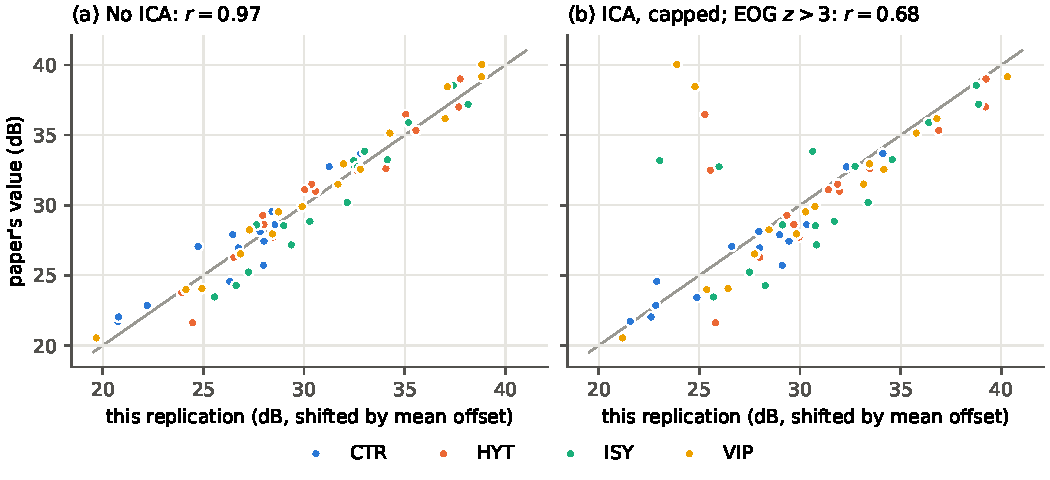
\includegraphics[width=0.85\linewidth]{figures/matched_per_subject.pdf}
\caption{Per-subject parieto-occipital gamma in MED: this replication against the paper's values from Zenodo
(63 subjects). This replication's values are shifted by the mean offset between the two scales.}
\label{fig:persubject}
\end{figure}

\paragraph{Group differences on the parieto-occipital cluster.} Fig.~\ref{fig:headline} gives the
group differences on the 8-electrode cluster mean, with Welch $t$-tests, for the paper's values and for both
pipelines; Table~\ref{tab:roi} (Appendix~\ref{app:tables}) lists the values.
\begin{itemize}
  \item \textbf{Gamma, no ICA.} Each meditator group exceeds controls by 3.5--4.8\,dB in MED and as a trait, all
        with $p \le .02$. These are within 1\,dB of the paper's own values for every contrast.
  \item \textbf{Gamma, automated ICA.} The differences shrink by about 1\,dB on average. VIP is affected most
        (MED: $+2.6$\,dB, $p = .12$; trait: $+2.4$\,dB, $p = .09$), while HYT and ISY stay significant. Pooled
        meditators still exceed controls in MED ($+3.1$\,dB, $p = .011$) and as a trait ($+3.3$\,dB, $p = .002$).
  \item \textbf{Alpha.} VIP has more alpha than controls in MED in all three sources (3.5--4.3\,dB,
        $p \le .014$), and more than HYT and ISY combined (about 4\,dB, $p \le .007$). The effect is weaker in IMW
        ($p = .03$--$.07$ in this replication).
\end{itemize}
So this replication largely confirms the paper's findings in these areas, with some attenuation 
of estimates when using the automated ICA pipeline.

\begin{figure}[htbp]
\centering
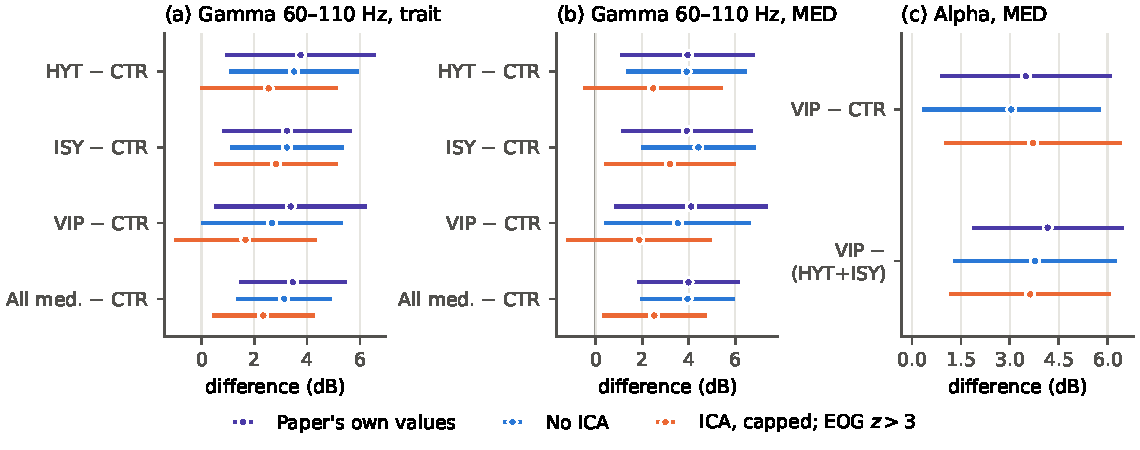
\includegraphics[width=\linewidth]{figures/matched_headline.pdf}
\caption{Group differences on the parieto-occipital cluster with 95\% confidence intervals (Welch), for the
paper's values and both pipelines.}
\label{fig:headline}
\end{figure}

\paragraph{Cluster permutation tests.} Table~\ref{tab:clusters} gives the smallest cluster $p$-value for each
electrode-level test, following the paper's procedure (Appendix~\ref{app:clusters}, where the topographies are
shown). All clusters with $p < .05$ are positive: meditators above controls in gamma, VIP above the other groups
in alpha.
\begin{itemize}
  \item \textbf{Gamma, no ICA.} All three groups have a significant cluster against controls in MED
        ($p = .017$, $.024$, $.042$ for HYT, ISY, VIP). As a trait, HYT and ISY do ($p = .029$, $.032$) and VIP
        narrowly misses ($p = .055$). The clusters are centred on parieto-occipital electrodes; for HYT and the pooled
        meditators in MED they extend over most of the scalp (43 electrodes).
  \item \textbf{Gamma, automated ICA.} Only ISY keeps a significant MED cluster ($p = .042$, 9 parieto-occipital
        electrodes). HYT and ISY remain significant as a trait and in IMW, and VIP has no cluster below $p = .13$
        in any condition.
  \item \textbf{Alpha.} In MED, VIP exceeds controls, HYT and ISY in both pipelines ($p = .013$--$.040$), with
        broad clusters of 46--59 electrodes. In IMW, VIP exceeds HYT in both pipelines and exceeds controls only
        with ICA ($p = .023$).
  \item \textbf{MED vs IMW within groups.} No group shows a significant difference between conditions in either
        band (smallest $p = .12$).
\end{itemize}
So the cluster permutation tests largely replicate the paper's findings, with some differences 
depending on the pipeline used, but nothing that fundamentally contradicts the original findings.

\begin{table}[htbp]
\centering\small
\begin{tabular}{@{}llcccccc@{}}
\toprule
 & & \multicolumn{3}{c}{No ICA} & \multicolumn{3}{c}{Capped ICA} \\
\cmidrule(lr){3-5}\cmidrule(lr){6-8}
Band & Contrast & MED & IMW & trait & MED & IMW & trait \\
\midrule
Gamma & HYT $-$ CTR & \textbf{.017} (43) & \textbf{.042} (23) & \textbf{.029} (40) & .066 (5) & \textbf{.038} (26) & \textbf{.034} (26) \\
 & ISY $-$ CTR & \textbf{.024} (32) & .059 (9) & \textbf{.032} (22) & \textbf{.042} (9) & \textbf{.035} (21) & \textbf{.032} (18) \\
 & VIP $-$ CTR & \textbf{.042} (19) & .114 (4) & .055 (11) & .179 (1) & .190 (1) & .136 (1) \\
 & All meditators $-$ CTR & \textbf{.021} (43) & \textbf{.040} (19) & \textbf{.033} (36) & .053 (10) & \textbf{.034} (28) & \textbf{.041} (22) \\
\midrule
Alpha & VIP $-$ CTR & \textbf{.031} (48) & .065 (14) & \textbf{.034} (43) & \textbf{.013} (59) & \textbf{.023} (54) & \textbf{.017} (59) \\
 & VIP $-$ HYT & \textbf{.022} (59) & \textbf{.029} (45) & \textbf{.025} (54) & \textbf{.033} (47) & \textbf{.033} (44) & \textbf{.034} (46) \\
 & VIP $-$ ISY & \textbf{.038} (46) & .076 (8) & .056 (28) & \textbf{.040} (46) & -- & .089 (4) \\
 & All meditators $-$ CTR & -- & -- & -- & -- & -- & -- \\
\bottomrule
\end{tabular}

\caption{Cluster permutation tests over electrodes: smallest cluster $p$-value, with the number of electrodes in
that cluster in brackets; $p < .05$ in bold; -- means no electrode passed the cluster-forming threshold. Two-tailed,
2000 permutations, 63 subjects.}
\label{tab:clusters}
\end{table}

\paragraph{Correcting for the number of tests.} The paper's cluster tests correct across electrodes within each
test, but not across the many tests run. To see whether this matters, we applied a Benjamini--Hochberg false
discovery rate (FDR) correction (Benjamini and Hochberg, 1995) at 5\% to each test's smallest cluster $p$-value, within each pipeline. 
The family of tests is the 23 tests that correspond to claims in the paper: gamma, each
tradition against controls in MED, IMW and trait; alpha, VIP against each other group in MED and IMW; MED against
IMW within each group in both bands.
\begin{itemize}
  \item In each pipeline, 10 of the paper's 23 tests reach $p < .05$, against about 1 expected if there were no
        effects at all.
  \item None survive the FDR correction, in either pipeline. The smallest adjusted $p$-value is $q = .097$
        over the paper's tests in both pipelines, and $.106$ (no ICA) and $.114$ (capped ICA) when all 38 tests run here
        are included.
  \item The reason is that every significant cluster $p$-value lies between $.013$ and $.042$. Benjamini--Hochberg
        needs the $k$-th smallest of $m$ $p$-values to be at most $0.05\,k/m$; with 10 hits out of 23, the 10th
        would need to be below $.022$.
\end{itemize}
However, a 10\% FDR correction would keep all of them, so the results are clearly not entirely spurious. A reasonable
conclusion is that the paper's reported p-values slightly overstate their statistical significance, but
their main conclusions are not entirely undermined.

\paragraph{Gamma and meditation experience.} The paper reports a skipped correlation of $r = 0.33$
(95\% CI [0.06, 0.53]) between meditators' trait parieto-occipital gamma and log lifetime practice hours (its
Fig.~4D). We reimplemented the skipped correlation (Pernet, Wilcox and Rousselet, 2013): bivariate outliers are
detected with the projection method and removed, and Pearson's $r$ is computed on the rest. Results are in
Table~\ref{tab:experience} and Fig.~\ref{fig:experience}.
\begin{itemize}
  \item \textbf{The point estimate reproduces exactly.} On the paper's values for its 48 meditators, two outliers
        are removed (HYT7, with many hours and low gamma; ISY6, with few hours and high gamma), giving $r = 0.33$.
        Without the outlier step the correlation is weak: Pearson $r = 0.16$ ($p = .27$).
  \item \textbf{The confidence interval depends on how the bootstrap treats the outliers.} If the two outliers are
        removed once and Pearson's $r$ is bootstrapped on the remaining 46 meditators, the 95\% CI is [0.08, 0.54],
        matching the paper's up to monte carlo error. This is presumably what the paper did. 
        It ignores the uncertainty in which points get flagged as outliers. Redoing the outlier detection within 
        each bootstrap resample gives [$-0.14$, 0.51],
        which includes zero.
  \item \textbf{The estimate is fragile.} Dropping HYT26, the one meditator missing from \texttt{ds003969},
        changes which points are flagged as outliers and lowers $r$ to 0.24.
  \item \textbf{This replication's own gamma shows no clear relationship:} $r = 0.16$ without ICA (no outliers
        flagged) and $r = -0.05$ with capped ICA. Both CIs include zero under either bootstrap approach.
\end{itemize}

Overall this suggests that the reported correlation between trait parieto-occipital gamma and 
meditation experience is extremely sensitive to outlier handling. Visually, considering figure \ref{fig:experience}a, 
which is an exact replication of the paper's figure 4D, it's clear that the slope of the fitted
line is driven by the choice to remove two outliers.

\begin{table}[htbp]
\centering\small
\begin{tabular}{@{}lrrrlcc@{}}
\toprule
 & & & & & \multicolumn{2}{c}{95\% CI, outliers\ldots} \\
\cmidrule(l){6-7}
Gamma values & $n$ & Pearson $r$ & Skipped $r$ & Outliers & removed once & redetected \\
\midrule
Paper\textquotesingle s values & 48 & 0.16 & 0.33 & HYT7 ISY6 & [0.08, 0.54] & [$-$0.14, 0.51] \\
\quad without HYT26 & 47 & 0.17 & 0.24 & HYT7 & [$-$0.07, 0.50] & [$-$0.17, 0.50] \\
\midrule
No ICA & 47 & 0.16 & 0.16 & none & [$-$0.16, 0.45] & [$-$0.19, 0.51] \\
Capped ICA & 47 & 0.06 & $-$0.05 & HYT20 & [$-$0.36, 0.27] & [$-$0.34, 0.34] \\
\midrule
Paper (Fig.~4D) & 48 & & 0.33 & & [0.06, 0.53] & \\
\bottomrule
\end{tabular}

\caption{Correlation between trait parieto-occipital gamma and $\log_{10}$ lifetime practice hours among meditators.
Skipped correlations with percentile bootstrap CIs (2000 resamples). ``Removed once'' bootstraps Pearson's
$r$ on the subjects left after removing the outliers found in the full sample; ``redetected'' repeats the outlier
detection in each resample. The upper rows use the paper's values, for all 48 meditators and for the 47 in
\texttt{ds003969}; the lower rows use this replication's values. Practice hours are from the paper's Zenodo file.}
\label{tab:experience}
\end{table}

\begin{figure}[htbp]
\centering
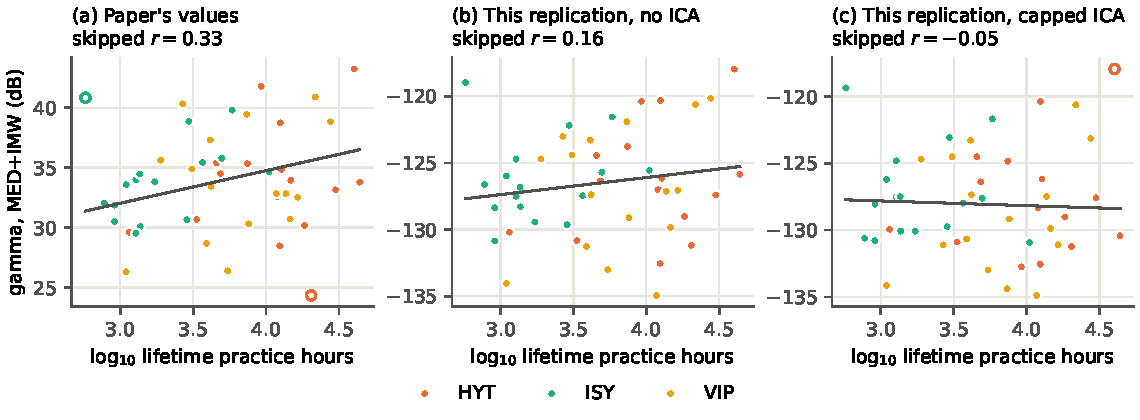
\includegraphics[width=\linewidth]{figures/experience_gamma.pdf}
\caption{Trait parieto-occipital gamma against lifetime practice hours (the paper's Fig.~4D). Open circles are the
outliers removed by the skipped correlation; lines are fitted to the remaining points.}
\label{fig:experience}
\end{figure}

\subsection{Criticality}
\label{sec:critresults}

The main reported results here are for the pipeline that uses automated ICA component removal. 
All analysis was also run with the no-ICA pipeline and 
the results were qualitatively similar, with close point estimates and no major differences in significance.

Mean DFA exponents were above 0.5 in every band (0.74 in alpha, 0.69 in beta and 0.80 in gamma), 
indicating long-range temporal correlations in the amplitude envelopes. Mean fEI was below 1 in every band (0.93 in
alpha, 0.85 in beta and 0.91 in gamma), which in the fEI framework indicates slightly inhibition-dominated dynamics.
Hypotheses
were tested using OLS regressions of the subject-level DFA exponent (and, for $H_1$, fEI) with standard errors
clustered by subject. In each model, we also include an indicator variable for being in the second pair of tasks
 as a control for reasons outlined in section~\ref{sec:critmethod}. 
Fig.~\ref{fig:crit} shows the key terms, and Tables~\ref{tab:h1} and~\ref{tab:h2}
(Appendix~\ref{app:tables}) give the full estimates.

\paragraph{$H_1$: no trait difference between groups.} The trait measure uses \texttt{med2} and \texttt{think2},
as in the spectral analysis: 72 recordings from 49 subjects.
\begin{itemize}
  \item \textbf{DFA.} No meditator group differs from controls in any band (all $p \ge .15$). A joint test that all
        four groups are equal gives $p = .74$ (alpha), $.37$ (beta) and $.86$ (gamma). This is consistent with $H_1$,
        and with Lewis-Healey et al.\ (2026). The confidence intervals are wide, though ($\pm 0.07$--$0.10$ in alpha
        and beta, $\pm 0.11$--$0.16$ in gamma), so moderate group differences cannot be ruled out.
  \item \textbf{fEI.} Beta and gamma show no group differences (joint $p = .62$ and $.85$). In alpha, VIP has
        higher fEI than controls ($+0.20$, $p = .003$), and the joint test rejects equal groups ($p = .003$), so
        $H_1$ does not hold for alpha fEI. HYT and ISY do not differ from controls. This was unexpected but
        in ways aligns with the finding of higher alpha power in VIP. This result does not appear to be
        driven by outliers: alpha fEI lies above the control median for 11 of the 12 VIP subjects.
%   \item \textbf{It cannot be separated from alpha power.} VIP also has the highest alpha power
%         (Section~\ref{sec:power}), and fEI tracks alpha power closely. With power measured in the same band and
%         channels as fEI (8--13\,Hz, all good channels), the two correlate across subjects (Spearman $\rho = 0.59$,
%         $p < .001$), and within subjects fEI rises by 0.05 per dB of alpha power across their recordings
%         ($p < .001$). Adding trait alpha power to the regression reduces the VIP difference to $+0.13$ ($p = .08$).
%         This coupling could reflect a measurement effect, since fEI estimates depend on how strongly the oscillation
%         stands out from the background, or a shared mechanism, since a shift in excitation/inhibition balance would
%         change amplitude and its dynamics together. Either way, VIP's higher alpha fEI largely accompanies their higher
%         alpha power and cannot be distinguished from it in these data.
\end{itemize}
Interestingly, this fEI result mirrors the alpha power results: VIP shows higher alpha power than controls, 
while HYT and ISY do not differ from controls. Measuring alpha power in the same band as fEI (8--13\,Hz) 
we find a correlation of 0.59 ($p < .001$) between alpha power and alpha fEI across subjects. This is an interesting
relationship, and two explanations that cannot be distinguished by this data present themselves: it could be 
that higher alpha power drives observed increases in fEI (fEI estimates may depend on the prominence 
of the oscillation in the data), 
or that both are driven by a common underlying factor such as excitation/inhibition balance.

\paragraph{$H_2$: DFA increases during meditation.} This uses all four blocks for the meditators: 117 recordings
from 40 subjects.
\begin{itemize}
  \item \textbf{Beta DFA rises from \texttt{med1breath} to \texttt{med2}} ($+0.061$, $p = .009$). Alpha shows a
        smaller and less significant rise ($+0.039$, $p = .055$), and gamma none.
  \item \textbf{This rise cannot be separated from time on task.} \texttt{med2} always directly follows
        \texttt{med1breath}, so the first-to-second-block change also contains any generic effect of time spent in
        the task. The comparison with the thinking pair, (\texttt{med2} $-$ \texttt{med1breath}) $-$
        (\texttt{think2} $-$ \texttt{think1}), isolates the part specific to meditation. It has a similar point 
        estimate and is positive in beta ($+0.052$) but is not significant in any band (beta $p = .15$, 
        alpha $p = .63$, gamma $p = .97$).
\end{itemize}
So the data show an increase in beta DFA over the meditation session, in the direction $H_2$ predicts. However, there
is insufficient evidence to conclude that the increase is specifically due to meditation rather than a generic time
on task effect.

\paragraph{Session order.} DFA is lower in the second pair of blocks, after the break, in every band. The difference
is significant in beta ($-0.052$, $p = .044$ in the $H_1$ model; $-0.043$, $p = .014$ in the $H_2$ model) and
close to significance in alpha ($p = .09$ in both). Subjects completed a questionnaire and a set of auditory and visual tasks between 
the first and second 
pairs of blocks. Braboszcz et al. (2017) mention these tasks but do not report their results. It's possible these tasks were responsible for the observed session order effect.

\paragraph{Without ICA.} Appendix Fig.~\ref{fig:critnoica} repeats both analyses on the no-ICA pipeline. The
results do not differ: no DFA estimate changes by more than 0.02 and no fEI estimate by more than 0.04. The only
term that changes significance is VIP $-$ CTR in beta fEI ($+0.09$, $p = .043$ without ICA; $+0.05$, $p = .25$
with ICA); the alpha fEI difference holds in both ($p = .005$ without ICA).

As noted in section \ref{sec:critmethod}, the choice to use base 180 second epochs for the criticality analysis 
means a lot of data is dropped, with only 59\% of recordings having at least one usable epoch. To test
the robustness of these results to that choice, we reran this analysis using 90 second epochs. This resulted in 
88\% of recordings having at least one usable epoch. The main results above 
(No group differences in DFA, higher trait fEI for VIP practitioners, and a positive change in beta DFA over the meditation session)
 all survived this change. 

\begin{figure}[htbp]
\centering
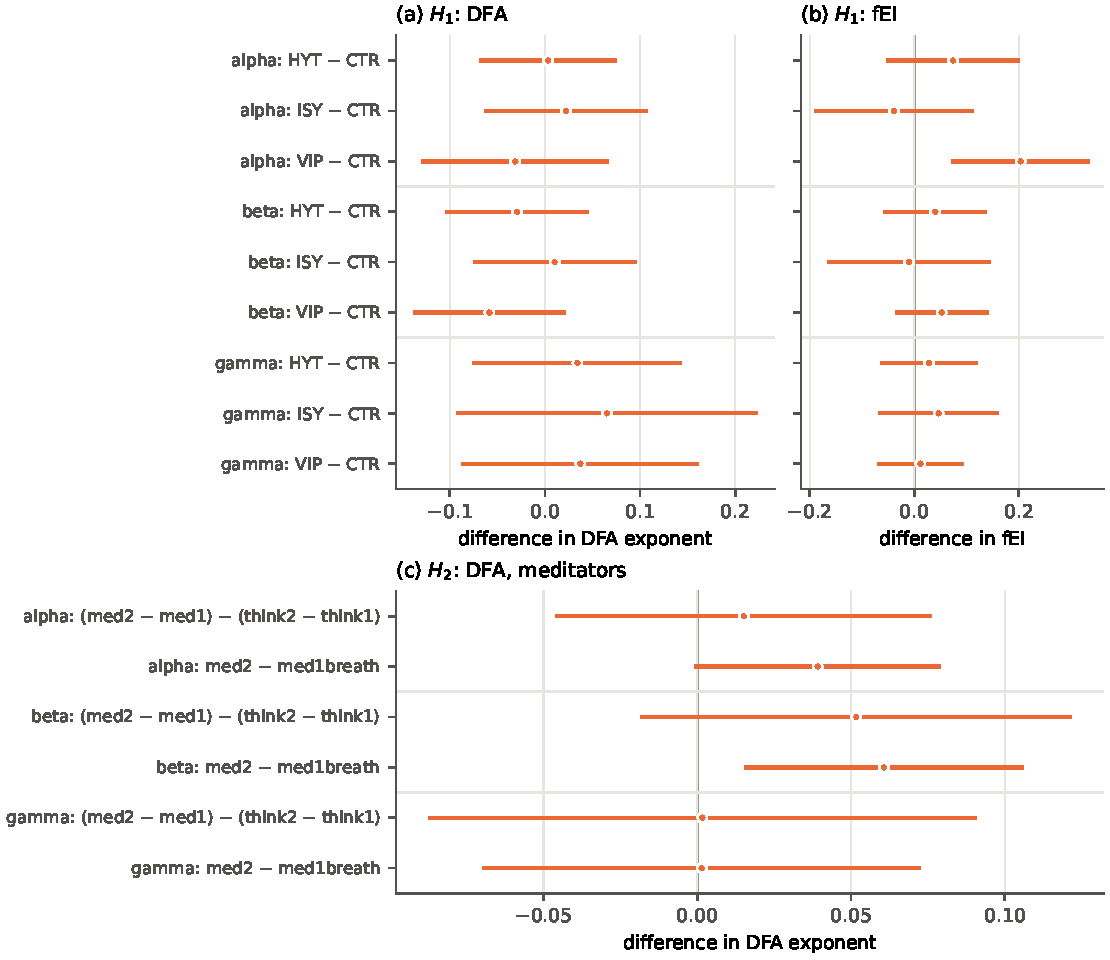
\includegraphics[width=\linewidth]{figures/criticality_final.pdf}
\caption{Key terms from the criticality regressions (capped ICA), with 95\% confidence intervals. (a, b) Each meditator
group against controls, \texttt{med2} and \texttt{think2}, for DFA and fEI. (c) Within meditators: the change from \texttt{med1breath}
to \texttt{med2}, and that change minus the change from \texttt{think1} to \texttt{think2}.}
\label{fig:crit}
\end{figure}

%-------------------------------------------------------------------------------
\section{Conclusion}

Here we have largely replicated the data processing pipeline and analysis
of Braboszcz et al. (2017). As a learning exercise this has been very fruitful, covering 
the early stages of EEG data processing through to the final statistical analyses. 

In constructing the pipeline, the main difficulty in replicating the original design
was steps that required unspecified manual intervention, such as artifact rejection and channel selection.
Ultimately it was not possible to exactly replicate the processing and fortunately it was not necessary,
as all analysis shown above was largely robust to different choices made during preprocessing.
Really this is a better outcome than an exact replication as we actually learn something
about the robustness of the original findings.

The authors' (Braboszcz et al., 2017) results on gamma power in meditators and alpha power specifically in 
vipassana practitioners both replicate and do so robustly to different choices made in the 
preprocessing pipeline. However, their result on the relationship between gamma power and lifetime hours 
of meditative practice has been shown to be extremely fragile, depending entirely on the 
choice to drop two observations as outliers.

A further analysis of criticality metrics (DFA and fEI) found no trait differences in DFA between
controls or meditators of any type, consistent with the findings of Lewis-Healey et al. (2026).
However, there is some evidence for higher trait alpha fEI specifically in vipassana practitioners. 
This aligns with the finding of higher alpha power for this group, and the two findings are difficult to separate.
There was some suggestive evidence for criticality increasing for meditators during meditation, 
although the estimation procedure could not distinguish whether this was an effect of meditation
or a more generic time on task effect.




\clearpage

\section*{References}
\begingroup
\small
\begin{itemize}[label={}, leftmargin=1.6em, itemindent=-1.6em, itemsep=0.5em]
  \item Benjamini Y, Hochberg Y (1995). Controlling the false discovery rate: a practical and powerful approach to
        multiple testing. \emph{Journal of the Royal Statistical Society: Series B} \textbf{57}(1): 289--300.
        \doi{10.1111/j.2517-6161.1995.tb02031.x}
  \item Braboszcz C, Cahn BR, Levi J, Fernandez M, Delorme A (2016). Data files related to the article ``Different
        meditation practices share the same neuronal correlates: increased gamma brainwave amplitude compared to
        control in three different meditation traditions''. \emph{Zenodo} [dataset]. \doi{10.5281/zenodo.57911}
  \item Braboszcz C, Cahn BR, Levy J, Fernandez M, Delorme A (2017). Increased gamma brainwave amplitude compared to
        control in three different meditation traditions. \emph{PLoS ONE} \textbf{12}(1): e0170647.
        \doi{10.1371/journal.pone.0170647}
  \item Bruining H, Hardstone R, Juarez-Martinez EL, Sprengers J, Avramiea AE, Simpraga S, et al.\ (2020).
        Measurement of excitation-inhibition ratio in autism spectrum disorder using critical brain dynamics.
        \emph{Scientific Reports} \textbf{10}: 9195. \doi{10.1038/s41598-020-65500-4}
  \item Delorme A, Braboszcz C (2021). Meditation vs thinking task. \emph{OpenNeuro} [dataset], \texttt{ds003969}
        v1.0.0. \doi{10.18112/openneuro.ds003969.v1.0.0}
  \item Hardstone R, Poil SS, Schiavone G, Jansen R, Nikulin VV, Mansvelder HD, Linkenkaer-Hansen K (2012).
        Detrended fluctuation analysis: a scale-free view on neuronal oscillations. \emph{Frontiers in Physiology}
        \textbf{3}: 450. \doi{10.3389/fphys.2012.00450}
  \item Lewis-Healey E, Kringelbach M, Canales-Johnson A, Laukkonen R (2026). Near-critical brain dynamics track
        effortlessness during meditation. \emph{bioRxiv} [preprint]. \doi{10.64898/2026.08.07.743470}
  \item Linkenkaer-Hansen K, Nikouline VV, Palva JM, Ilmoniemi RJ (2001). Long-range temporal correlations and
        scaling behavior in human brain oscillations. \emph{Journal of Neuroscience} \textbf{21}(4): 1370--1377.
        \doi{10.1523/JNEUROSCI.21-04-01370.2001}
  \item Pernet CR, Wilcox R, Rousselet GA (2013). Robust correlation analyses: false positive and power validation
        using a new open source Matlab toolbox. \emph{Frontiers in Psychology} \textbf{3}: 606.
        \doi{10.3389/fpsyg.2012.00606}
\end{itemize}
\endgroup

\clearpage

\appendix
\section{Cluster permutation tests}
\label{app:clusters}

The electrode-level tests follow the paper's description of its FieldTrip analysis:
\begin{itemize}
  \item \textbf{Power per electrode.} Median over 1\,Hz bins of $10\log_{10}$ power in the band. Bad channels were
        interpolated with spherical splines so that every subject has a value at every electrode.
  \item \textbf{Statistic.} Student's $t$ at each electrode: independent samples for group comparisons, paired for
        MED against IMW within a group.
  \item \textbf{Clusters.} Electrodes with $|t|$ above the two-tailed $p < .05$ threshold are grouped with
        neighbouring electrodes (Delaunay triangulation of the 64-channel layout). Each cluster is scored by its
        summed $t$.
  \item \textbf{Inference.} Group labels were shuffled 2000 times (sign flips for the paired tests), recording the
        largest cluster score each time. A cluster's $p$-value is the proportion of permutations whose largest score
        is at least as large. This controls the family-wise error rate across electrodes within each test, but not
        across tests.
\end{itemize}
Figures~\ref{fig:clustergamma} and~\ref{fig:clusteralpha} show the group differences, with the electrodes in
clusters with $p < .05$ marked.
The code is in \nolinkurl{code/cluster_stats.py} and \nolinkurl{scripts/cluster_tests.py}, and the results are in
\nolinkurl{results/matched/cluster_tests.csv} and, with FDR-adjusted values, \nolinkurl{cluster_tests_fdr.csv}.

\begin{figure}[p]
\centering
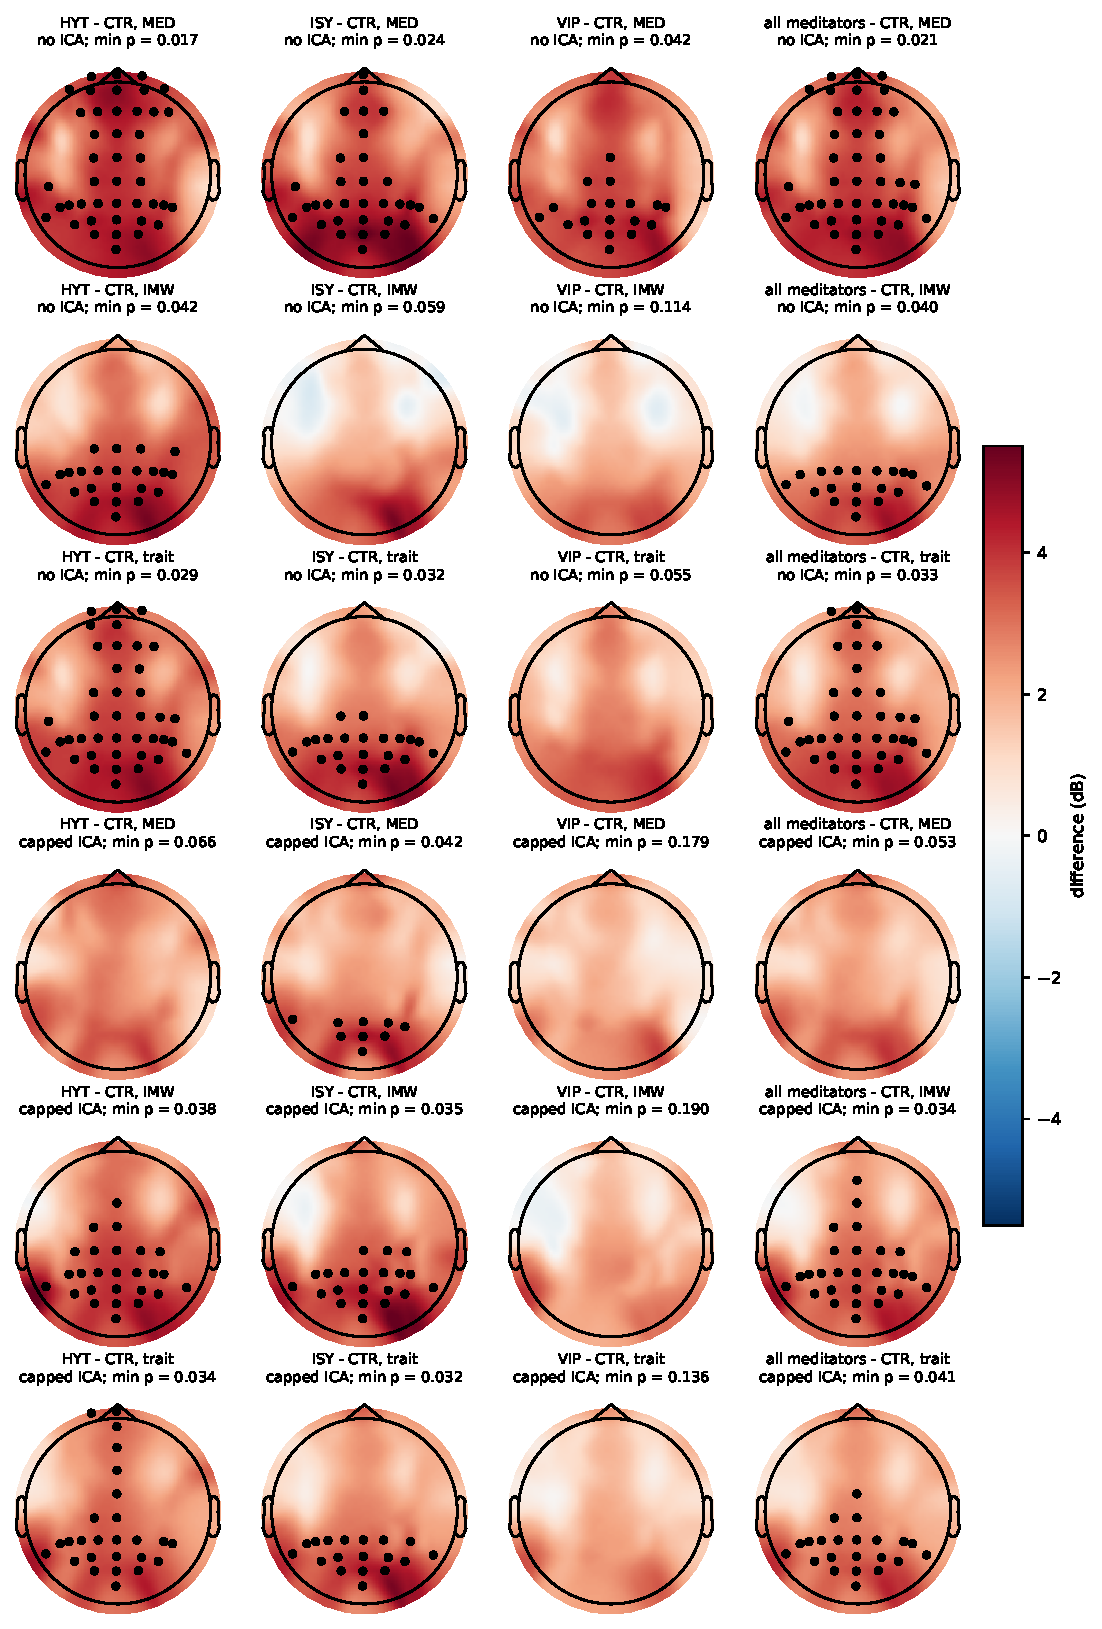
\includegraphics[width=0.9\linewidth]{figures/cluster_gamma.pdf}
\caption{Gamma (60--110\,Hz): mean difference from controls (dB). Black dots mark electrodes in clusters with
$p < .05$. Rows 1--3: no ICA; rows 4--6: capped ICA.}
\label{fig:clustergamma}
\end{figure}

\begin{figure}[p]
\centering
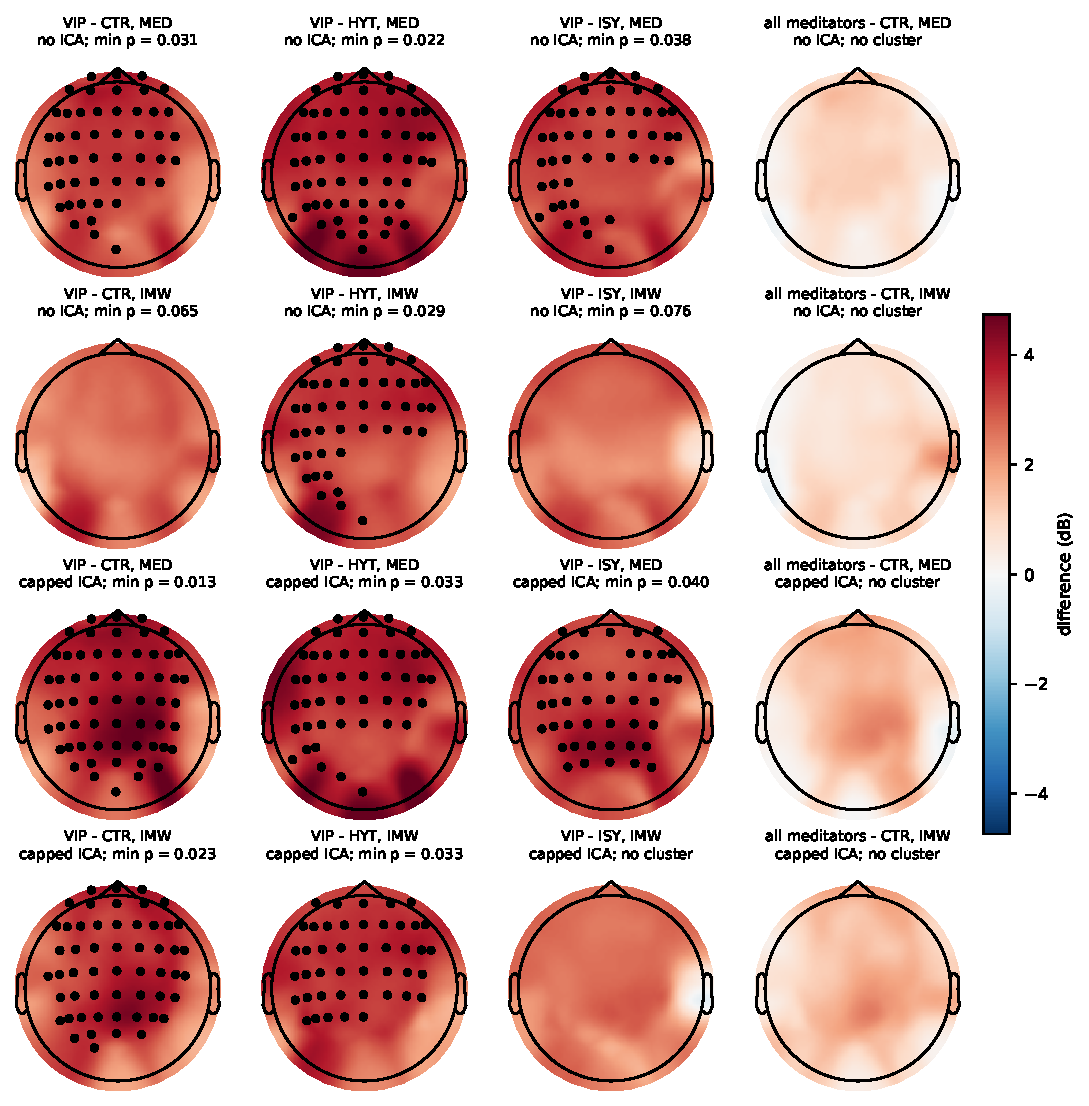
\includegraphics[width=0.9\linewidth]{figures/cluster_alpha.pdf}
\caption{Alpha (7--11\,Hz): VIP compared with each other group, and all meditators against controls (dB). Black
dots mark electrodes in clusters with $p < .05$. Rows 1--2: no ICA; rows 3--4: capped ICA.}
\label{fig:clusteralpha}
\end{figure}

\clearpage
\section{Criticality without ICA}

\begin{figure}[H]
\centering
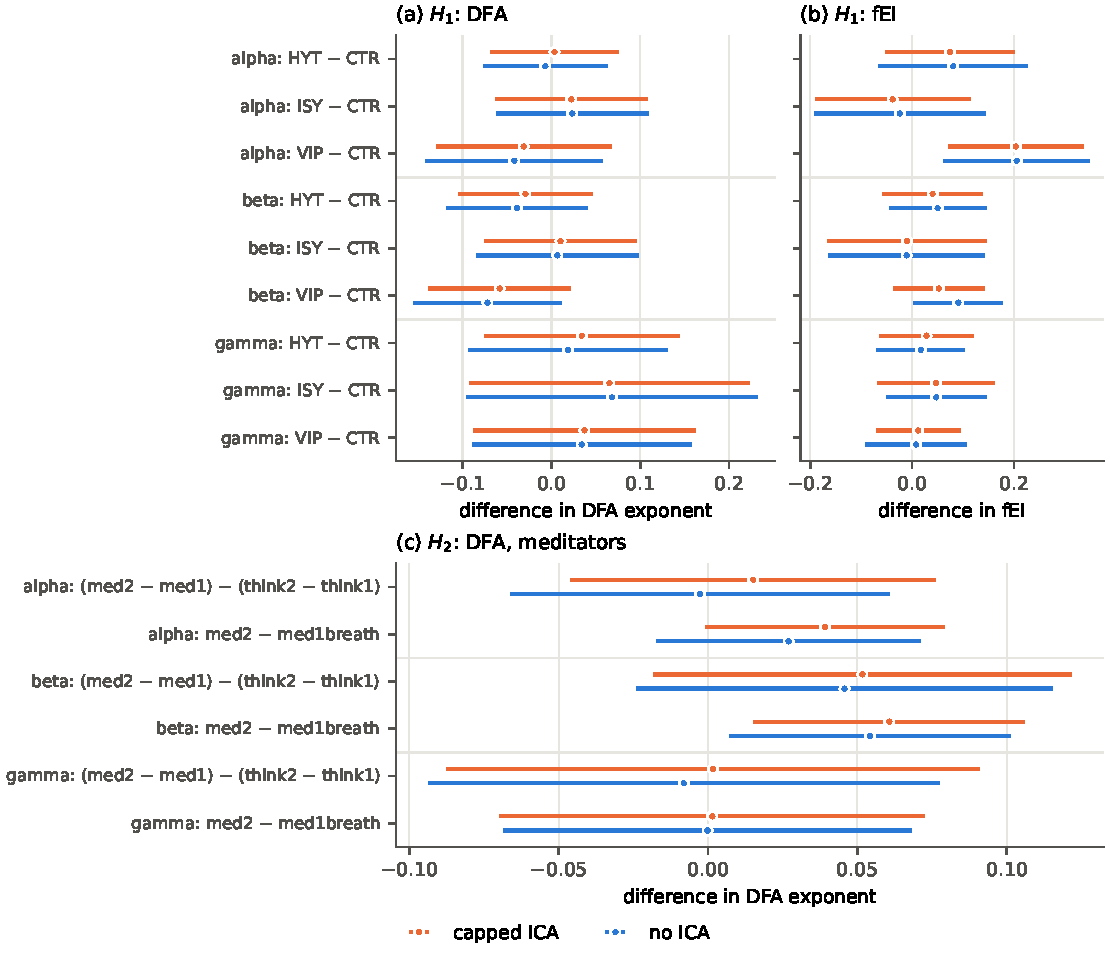
\includegraphics[width=\linewidth]{figures/criticality_final_noica.pdf}
\caption{The terms in Fig.~\ref{fig:crit} for the capped-ICA pipeline (orange) and the no-ICA pipeline (blue), with
95\% confidence intervals.}
\label{fig:critnoica}
\end{figure}

\section{The paper's spectra}

\begin{figure}[H]
\centering
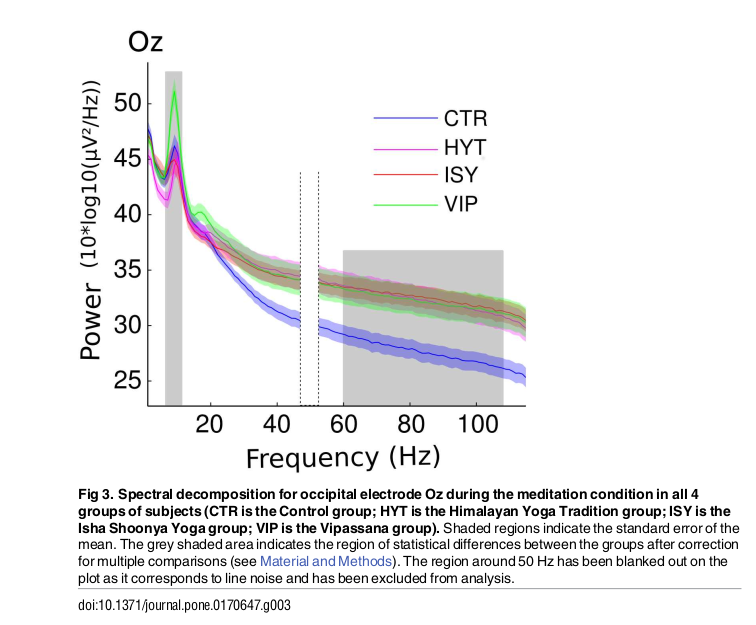
\includegraphics[width=0.6\linewidth]{figures/paper_fig3.png}
\caption{Braboszcz et al.\ (2017), Fig.~3: Oz spectra by group (CC BY 4.0).}
\label{fig:paper}
\end{figure}

\section{Full results tables}
\label{app:tables}

\begin{table}[H]
\centering\small
\begin{tabular}{@{}lllrrr@{}}
\toprule
Band & Condition & Contrast & Paper\textquotesingle s values & No ICA & Capped ICA \\
\midrule
Gamma 60--110\,Hz & MED & HYT $-$ CTR & +3.95 (\textbf{.012}) & +4.21 (\textbf{.006}) & +3.28 (\textbf{.042}) \\
 &  & ISY $-$ CTR & +3.92 (\textbf{.011}) & +4.80 (\textbf{$<$.001}) & +3.55 (\textbf{.022}) \\
 &  & VIP $-$ CTR & +4.10 (\textbf{.023}) & +4.12 (\textbf{.018}) & +2.55 (.123) \\
 &  & All meditators $-$ CTR & +3.99 (\textbf{.001}) & +4.38 (\textbf{$<$.001}) & +3.12 (\textbf{.011}) \\
 & IMW & HYT $-$ CTR & +3.56 (\textbf{.035}) & +4.26 (\textbf{.006}) & +3.90 (\textbf{.008}) \\
 &  & ISY $-$ CTR & +2.57 (.076) & +3.66 (\textbf{.005}) & +4.18 (\textbf{.001}) \\
 &  & VIP $-$ CTR & +2.66 (.071) & +2.82 (\textbf{.048}) & +2.26 (.110) \\
 &  & All meditators $-$ CTR & +2.93 (\textbf{.013}) & +3.56 (\textbf{.001}) & +3.44 (\textbf{.001}) \\
 & trait & HYT $-$ CTR & +3.76 (\textbf{.016}) & +4.23 (\textbf{.004}) & +3.59 (\textbf{.013}) \\
 &  & ISY $-$ CTR & +3.24 (\textbf{.014}) & +4.23 (\textbf{$<$.001}) & +3.87 (\textbf{.002}) \\
 &  & VIP $-$ CTR & +3.38 (\textbf{.029}) & +3.47 (\textbf{.020}) & +2.41 (.087) \\
 &  & All meditators $-$ CTR & +3.46 (\textbf{.002}) & +3.97 (\textbf{$<$.001}) & +3.28 (\textbf{.002}) \\
\midrule
Alpha 7--11\,Hz & MED & VIP $-$ CTR & +3.49 (\textbf{.014}) & +3.82 (\textbf{.013}) & +4.30 (\textbf{.006}) \\
 &  & VIP $-$ (HYT+ISY) & +4.16 (\textbf{.001}) & +4.24 (\textbf{.004}) & +4.08 (\textbf{.007}) \\
 & IMW & VIP $-$ CTR & +2.72 (\textbf{.047}) & +2.85 (.058) & +3.07 (.056) \\
 &  & VIP $-$ (HYT+ISY) & +3.43 (\textbf{.008}) & +3.23 (\textbf{.029}) & +2.79 (.071) \\
\bottomrule
\end{tabular}

\caption{Group differences in mean power over the 8-electrode parieto-occipital cluster (dB), with Welch $t$-test
$p$-values in brackets; $p < .05$ in bold. ``Paper's values'' puts the paper's per-subject values from Zenodo
(Braboszcz et al., 2016) through the same tests. Trait is each subject's mean of MED and IMW.}
\label{tab:roi}
\end{table}

\begin{table}[H]
\centering\small
\begin{tabular}{@{}lrrrrrr@{}}
\toprule
 & \multicolumn{2}{c}{Alpha} & \multicolumn{2}{c}{Beta} & \multicolumn{2}{c}{Gamma} \\
\cmidrule(lr){2-3}\cmidrule(lr){4-5}\cmidrule(lr){6-7}
Term & Estimate (SE) & $p$ & Estimate (SE) & $p$ & Estimate (SE) & $p$ \\
\midrule
\multicolumn{7}{@{}l}{\textit{DFA exponent}} \\
HYT $-$ CTR & +0.003 (0.037) & .925 & $-$0.029 (0.038) & .445 & +0.034 (0.056) & .541 \\
ISY $-$ CTR & +0.022 (0.044) & .608 & +0.010 (0.044) & .815 & +0.065 (0.081) & .418 \\
VIP $-$ CTR & $-$0.031 (0.050) & .535 & $-$0.058 (0.041) & .155 & +0.037 (0.064) & .558 \\
Second pair & $-$0.045 (0.026) & .089 & $-$0.052 (0.026) & \textbf{.044} & $-$0.022 (0.030) & .475 \\
All groups equal & $\chi^2_3 = 1.25$ & .742 & $\chi^2_3 = 3.12$ & .373 & $\chi^2_3 = 0.75$ & .861 \\
Observations (subjects) & \multicolumn{2}{c}{72 (49)} & \multicolumn{2}{c}{72 (49)} & \multicolumn{2}{c}{72 (49)} \\
\midrule
\multicolumn{7}{@{}l}{\textit{fEI}} \\
HYT $-$ CTR & +0.074 (0.065) & .253 & +0.040 (0.050) & .424 & +0.028 (0.047) & .550 \\
ISY $-$ CTR & $-$0.038 (0.078) & .621 & $-$0.010 (0.079) & .899 & +0.047 (0.058) & .424 \\
VIP $-$ CTR & +0.204 (0.068) & \textbf{.003} & +0.053 (0.045) & .248 & +0.012 (0.042) & .778 \\
Second pair & $-$0.031 (0.033) & .352 & $-$0.029 (0.031) & .357 & +0.030 (0.034) & .384 \\
All groups equal & $\chi^2_3 = 13.67$ & \textbf{.003} & $\chi^2_3 = 1.79$ & .617 & $\chi^2_3 = 0.80$ & .849 \\
Observations (subjects) & \multicolumn{2}{c}{72 (49)} & \multicolumn{2}{c}{72 (49)} & \multicolumn{2}{c}{72 (49)} \\
\bottomrule
\end{tabular}

\caption{$H_1$: OLS of the DFA exponent and of fEI on group and the second-pair indicator, using \texttt{med2} and
\texttt{think2}, with standard errors clustered by subject. Group terms are differences from controls. ``All groups
equal'' is a Wald test of the three group terms. $p < .05$ in bold.}
\label{tab:h1}
\end{table}

\begin{table}[H]
\centering\small
\begin{tabular}{@{}lrrrrrr@{}}
\toprule
 & \multicolumn{2}{c}{Alpha} & \multicolumn{2}{c}{Beta} & \multicolumn{2}{c}{Gamma} \\
\cmidrule(lr){2-3}\cmidrule(lr){4-5}\cmidrule(lr){6-7}
Term & Estimate (SE) & $p$ & Estimate (SE) & $p$ & Estimate (SE) & $p$ \\
\midrule
MED $-$ IMW (first block) & $-$0.005 (0.026) & .851 & $-$0.013 (0.020) & .513 & $-$0.008 (0.034) & .824 \\
think2 $-$ think1 & +0.024 (0.029) & .412 & +0.009 (0.025) & .717 & $-$0.000 (0.033) & .995 \\
(med2 $-$ med1) $-$ (think2 $-$ think1) & +0.015 (0.031) & .627 & +0.052 (0.036) & .148 & +0.002 (0.046) & .971 \\
med2 $-$ med1breath & +0.039 (0.020) & .055 & +0.061 (0.023) & \textbf{.009} & +0.001 (0.036) & .968 \\
Second pair & $-$0.038 (0.023) & .089 & $-$0.043 (0.018) & \textbf{.014} & $-$0.041 (0.023) & .069 \\
Observations (subjects) & \multicolumn{2}{c}{117 (40)} & \multicolumn{2}{c}{117 (40)} & \multicolumn{2}{c}{117 (40)} \\
\bottomrule
\end{tabular}

\caption{$H_2$: OLS of the DFA exponent for meditators on task (MED or IMW), position in the pair (first or second
block), their interaction and the second-pair indicator, with standard errors clustered by subject. The first
three rows are model terms; ``med2 $-$ med1breath'' is the sum of the second and third. $p < .05$ in bold.}
\label{tab:h2}
\end{table}

\end{document}
